\documentclass{siproblemset}

\usepackage{multicol}
\usepackage{xcolor}

% SI Session Information
\course{MTH 1321}
\sessionnum{7}
\sessiondate{9/25/19}

\warmup{Concept Review}
\topic{Formal Definition of the Derivative}
\topic{Introduction to Derivative Uses}
\topic{Derivatives of Functions}
\cooldown{Look Back, Look Forward}

% Worksheet Information
\title{Definition of the Derivative}
\sections{Sections 3.1 and 3.2a}
\withnamespace

\begin{document}
    \maketitle
    
    \activity{Warmup}{Concept Overview}{Work with a \textbf{partner} to answer these questions. Try not to use your notes.}{15 minutes}
    
    \frq{What are the limit definitions of the derivative of $f(x)$ at $x=a$?}
    \smallsp
    
    \frq{What are the limit definitions of the derivative of $f(x)$?}
    \smallsp
    
    \frq{What must be true for a function $f$ to be differentiable at $x=a$?}
    \smallsp
    
    \frq{What does $f'(x)$ represent both numerically and graphically?}
    \smallsp
    
    \pagebreak
    \activity{Activity 1}{Limit Definition of the Derivative}{Make a \textbf{group of two or three, all with the same colored worksheets,} to answer your assigned question. Try not to use your notes.}{30 minutes}
    
    \begin{multipartquestion}
        Determine both $f'(2)$ and $f'(x)$, using a limit definition for each:
        \frq{$f(x)=x^3-3x^2$}
        \Largesp
        \frq{$f(x)=\sqrt{x^2+3}$}
        \Largesp
%        \pagebreak
%        \frq{$f(x)=\dfrac{1}{3x-2}$}
%        \Hugesp
%        \frq{$f(x)=x+x^{-1}$}
    \end{multipartquestion}
    \pagebreak

    \activity{Activity 2}{Tangent Lines}{Make a \textbf{{\em new} group of three, all with the different colored worksheets,} to answer these questions. Try not to use your notes.}{30 minutes}
    
    \begin{multipartquestion}
        Use the graph below to answer the following questions.
        
        \makebox[\width][c]{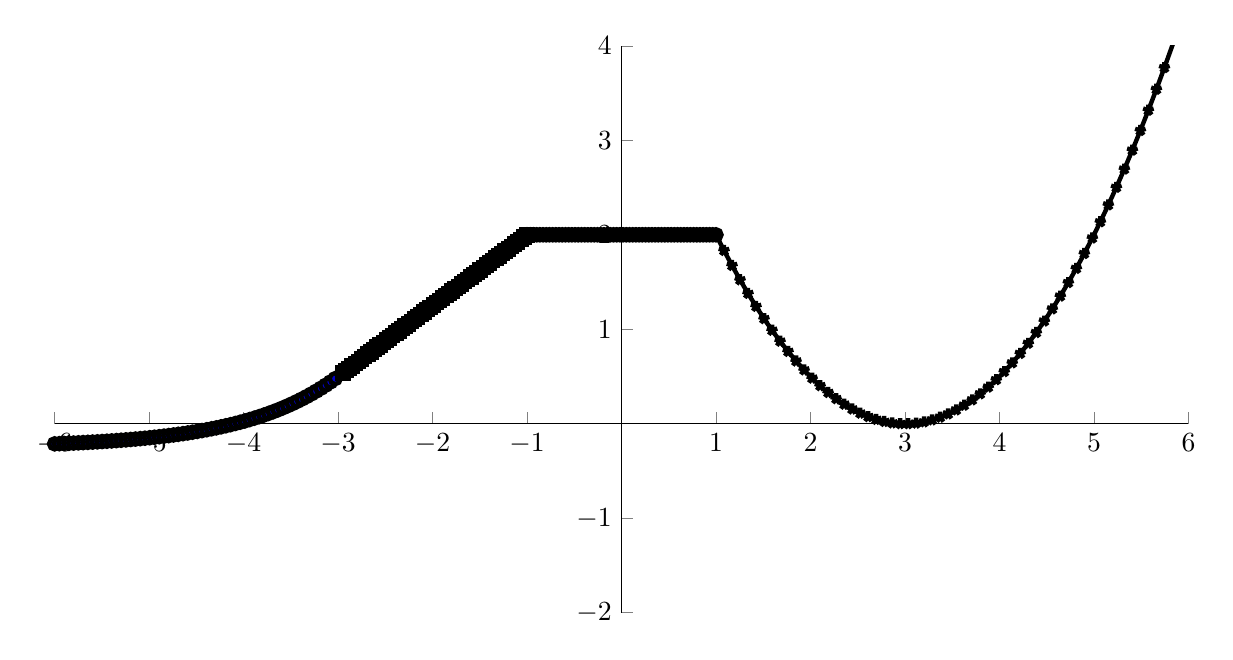
\begin{tikzpicture}[baseline=(current bounding box.north)]
            \begin{axis}[
            x=1.2cm,
            y=1.2cm,
            xmin=-6,
            xmax=6,
            ymin=-2,
            ymax=4,
            axis x line*=middle,
            axis y line*=middle,
            every axis plot/.append style={ultra thick},
            samples=60
            ]
            \addplot+[black, domain=-6:-3.03, restrict y to domain=-10:10] {e^(x+3+ln(3/4))-3/4+0.5};
            \addplot+[black, domain=-2.95:-1] {3/4*x+3/4+2};
            \addplot+[black, domain=-1:1] {2};
            \addplot+[black, domain=1:6] {1/2*(x-3)^2};
            \node at (-3,0.5) {$\circ$};
            \node at (-1,2) {\textbullet};
            \node at (1,2) {\textbullet};
            \end{axis}
            \end{tikzpicture}}
        \frq{Determine $f'(a)$ for $a=-3,-2,-1,0,1,3$. If $f$ is not differentiable at $x=a$, then state so explicitly.}
        \mediumspace
        \frq{Which is larger, $f'(2)$ or $f'(4)$? Justify your answer.}
        \nospace
        \frq{Which is larger, $|f'(2)|$ or $|f'(4)|$? Justify your answer.}
    \end{multipartquestion}
    \pagebreak
    
    
%    \frq{Use the limit definition of the derivative to compute $f'(a)$ when $a=4$. Then, find the equation of the tangent line to $f$ at $x=a$.}
%    $$f(x)=\frac{1}{2x+1}$$
%    \hugespace
%    \smallspace{\tiny \nospace}
    \pagebreak
    
    \activity{Cooldown}{Look Back, Look Forward}{Attempt to do these problems \textbf{alone} then discuss your answers with the people around you.}{15 minutes}
    \mcq[2]{What is the derivative of the following functions?}{
        \task $f(x)=mx+b$
        \task $g(t)=c$
    }
    \nospace
%    \frq{Determine the intervals when the derivative of the following function is positive, negative, and zero. If the derivative does not exist at an $x$-value, make sure to exclude it from all intervals.}
%    
%    \makebox[\width][c]{\begin{tikzpicture}[baseline=(current bounding box.north)]
%        \begin{axis}[
%        x=1.2cm,
%        y=1.2cm,
%        xmin=-6,
%        xmax=6,
%        ymin=-2,
%        ymax=4,
%        axis x line*=middle,
%        axis y line*=middle,
%        every axis plot/.append style={ultra thick},
%        samples=60
%        ]
%        \addplot+[black, domain=-6:-3.03, restrict y to domain=-10:10] {e^(x+3+ln(3/4))-3/4+0.5};
%        \addplot+[black, domain=-2.95:-1] {3/4*x+3/4+2};
%        \addplot+[black, domain=-1:1] {2};
%        \addplot+[black, domain=1:6] {1/2*(x-3)^2};
%        \node at (-3,0.5) {$\circ$};
%        \node at (-1,2) {\textbullet};
%        \node at (1,2) {\textbullet};
%        \end{axis}
%        \end{tikzpicture}}
%    \mediumspace
    
    \frq{When a function is increasing, it's derivative is \underline{\hspace{2in}}.}
    \tinysp
    \frq{When a function is decreasing, it's derivative is \underline{\hspace{2in}}.}
    \frq{Given the limit below, which represents $\dddx[f]$ at $x=x_0$, find $f(x)$ and $x_0$.}
    $$\lim\limits_{h\to 0}\frac{2e^{5+h}-2e^5}{h}$$
    \Smallsp
    
    \frq{Given the limit below, which represents $\dddf[g]{t}$ at $t=t_0$, find $g(t)$ and $t_0$.}
    $$\lim\limits_{t\to t_0}\frac{t^3+3t-{2}^3-3(2)}{t-2}$$
\end{document}